Para $\mathbf{F}(x,y)=\langle x+y,x\rangle$, construya una parametrización por tramos de la trayectoria mostrada y calcule su trabajo.
\begingroup
\shorthandoff{>}
\begin{center}
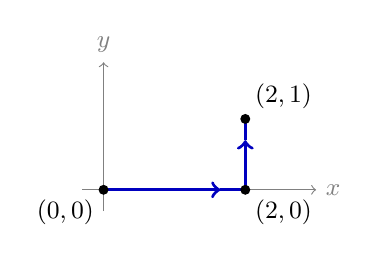
\begin{tikzpicture}[scale=.9,every node/.style={font=\small}]
    \draw[->,gray] (-.3,0)--(3,0) node[right] {$x$};
    \draw[->,gray] (0,-.3)--(0,1.8) node[above] {$y$};
    \draw[blue!75!black,very thick,->] (0,0)--(1.65,0);
    \draw[blue!75!black,very thick] (1.65,0)--(2,0);
    \draw[blue!75!black,very thick,->] (2,0)--(2,.7);
    \draw[blue!75!black,very thick] (2,.7)--(2,1);
    \fill (0,0) circle (2pt) node[below left] {$(0,0)$};
    \fill (2,0) circle (2pt) node[below right] {$(2,0)$};
    \fill (2,1) circle (2pt) node[above right] {$(2,1)$};
\end{tikzpicture}
\end{center}
\endgroup
